\documentclass[aps,pra,groupedaddress]{revtex4-1}
\usepackage{graphicx}
\usepackage{hyperref}
\usepackage{color}

%opening
\title{Bo Optical Simulation with RAT}
\author{Thomas Wester \\ \small{\href{https://github.com/tbwester/ratpac-nudot}{https://github.com/tbwester/ratpac-nudot}}}


\begin{document}

\maketitle

\begin{abstract}

\end{abstract}

\tableofcontents

\section{Introduction}

This note describes the optical photon simulation created to accompany measurements made with MicroBooNE PMTs in the Bo cryostat. The simulation uses RAT, a software package based around GEANT4, to handle the ray tracing and interaction properties of photons in the cryostat.

The simulation is divided into two steps: First, 128nm light is simulated as originating from scintillation in liquid argon induced by an alpha source. This light is propagated to an acrylic plate with a wavelength-shifting TPB coating. The position of the hits on this plate are saved. Second, 420nm light (representing wavelength-shifted photons) is created within the TPB plate and tracked through a glass volume representing the window of a MicroBooNE PMT. Photons which make it through this glass volume are recorded as successful hits.

\section{Geometry}

The Bo optical simulation uses the following convention: the positive $z$-direction points from the top of the cryostat towards the bottom, where the TPB plate and PMT are located. The $x$-$y$ plane is perpendicular and azimuthal symmetry is assumed. The origin is placed at the center (depth-wise and width-wise) of the cryostat volume. Every quantity listed in inches is converted to centimeters with the factor $2.54$. An overview of the geometry is shown in Figure \ref{fig:geo}.

\begin{figure}
	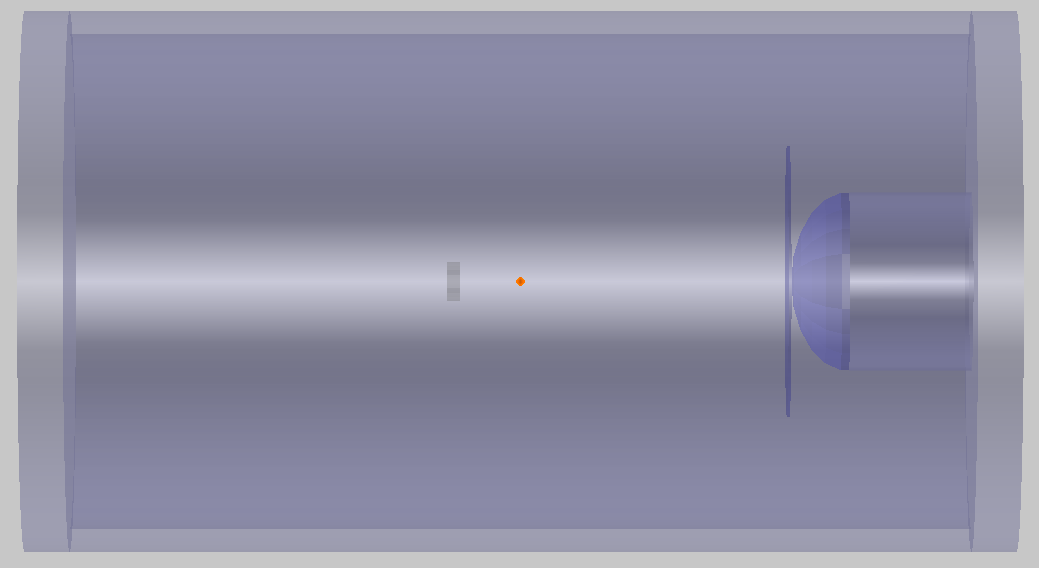
\includegraphics[width=1.0\textwidth]{figures/geo_overview}
	\caption{A view of the simulated Bo cryostat geometry showing (from left to right) the source holder, TPB plate, PMT glass and PMT metal shield. The origin in the simulation coordinate system is the orange point. \label{fig:geo}}
\end{figure}

\subsection{The Bo Cryostat}

The Bo cryostat is a cylindrical volume 40 inches in depth and 11 inches in inner-radius. Two end caps are placed with inner faces at $z=\pm 20$ inches to enclose the volume. 

\subsection{Source Holder}

The source holder is centered in the $x$-$y$ plane and is varied in position along the $z$-direction. The holder is modeled using three stacked ring volumes. A cross section is shown in Figure \ref{fig:holder}. The top two rings total in height to form the source collimator. The source itself is placed 0.01mm above the back of the collimator to simulate (i) the thickness of the aluminum foil on which the polonium is deposited and (ii) the potential for backscatters of photons reflecting on the aluminum.

There are two sets of measurements for the source holder. The first set, henceforth the ``primary'' set, has the height of the inner chamber at 0.09375 inches. The second configuration has this same height at 0.1 inches. In either case, the total depth of the collimator (0.15625") is the same.

\begin{figure}
	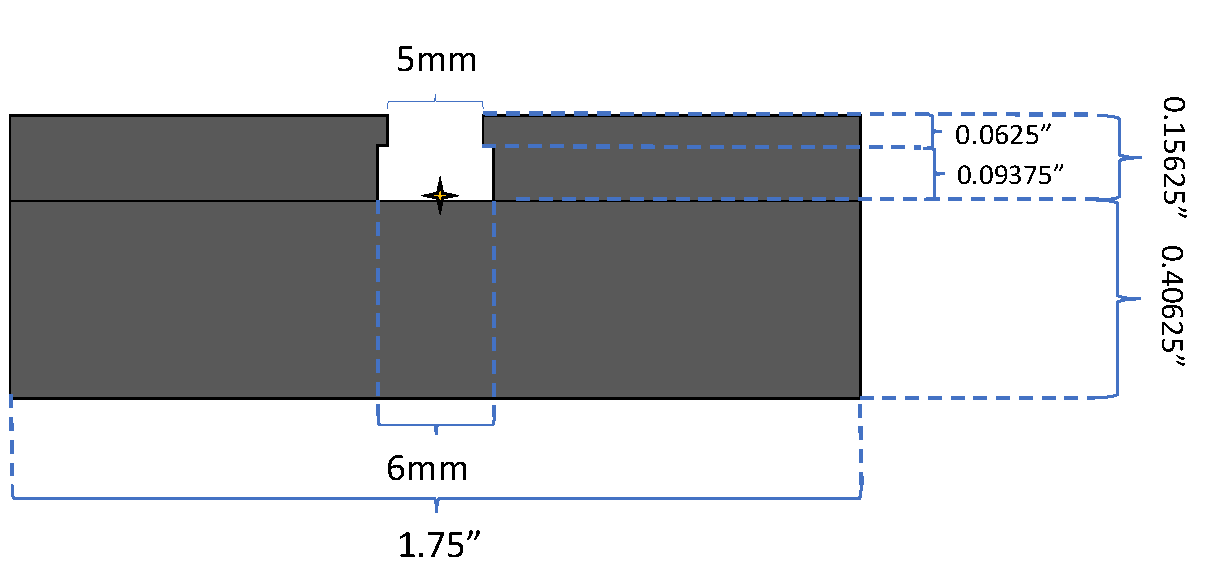
\includegraphics[width=1.0\textwidth]{figures/holder}
	\caption{To-scale cross-section of the source holder, with relevant dimensions labeled, using the primary source holder configuration. The source, indicated with a star, is placed just above the back of the collimator. \label{fig:holder}}
\end{figure}

\subsection{TPB Plate \& PMT}

The TPB plate is an acrylic disk 15.24 cm in radius and is placed such that the back face of the plate is 0.2cm in front of the PMT glass surface at its closest point. The plate is placed with its center at the origin in the $x$-$y$ plane and at a fixed position of $z=30$cm (front face).

\begin{table}
	\begin{center}
		\begin{tabular}{| c | c | c |}
			\hline
			Quantity & Value & Uncertainty \\
			\hline
			Cryostat Inner Radius & 11" & - \\
			Cryostat Depth & 40" & - \\
			Collimator Depth 1 & 0.0625" & - \\
			Collimator Depth 2 & 0.09375" & - \\
			Collimator Radius 1 & 2.5mm & - \\
			Collimator Radius 2 & 3mm & - \\
			TPB Plate Radius & 12" & - \\
			TPB Plate Depth & 0.125" & - \\
			PMT Glass Thickness & & - \\
			PMT Glass Major Axis & & - \\
			PMT Glass Minor Axis & & - \\
			\hline
		\end{tabular}
		\caption{Summary of relevant geometry parameters and associated uncertainties (where applicable). Note that the collimator has two associated radii and depths, see Figure \ref{fig:holder}. \label{tab:geo}}
	\end{center}
\end{table}

\begin{table}
	\begin{center}
		\begin{tabular}{| c | c | c |}
			\hline
			Feature & Position (cm) & Uncertainty \\
			\hline
			Cryostat Center & $(0,0,0)$ & - \\
			TPB Plate upper face & $(0,0,30)$ & - \\
			Source holder & Varies in $z$ & - \\
			\hline
		\end{tabular}
		\caption{Summary of geometry feature positions relative to the simulation origin. \label{tab:pos}}
	\end{center}
\end{table}

\section{Material Parameters}

This section describes the material properties relevant to the optical simulation. Table \ref{tab:mats} lists each simulation feature, its material, and the associated index of refraction, $N$, and reflectivity, $R$. Note that $N$ and $R$ have different values depending on the wavelength of the incident photon.

\begin{table}
	\begin{center}
		\begin{tabular}{| c | c | c | c |}
			\hline
			Feature & Material & $N$ (128/420nm) & $R$ (128/420nm) \\
			\hline
			Cryostat Walls & Stainless Steel & - & 0.35/0.55 \\
			Cryostat Interior & LAr & 1.33/1.23 & -\\
			Source Holder & Aluminum & - & 0.1 \cite{johnson_1968}\\
			TPB Plate & Acrylic & - & - \\
			PMT Window & Glass & - & - \\
			\hline
		\end{tabular}
		\caption{Summary of material properties relevant for the optical simulation. \label{tab:mats}}
	\end{center}
\end{table}

Additionally, we assign the Rayleigh scattering length parameter in LAr as $\lambda=60 \pm 6$ cm.

\section{Analysis}

\subsection{Rayleigh Scattering}

Rayleigh scattering has two properties relevant to the optical simulation. First, the probability of scattering is exponential with parameter $\lambda$. Second, the distribution of scattering angles, $\theta_s$, is proportional to $1+\cos^2 \theta_s$.

Both of these properties are implemented within RAT.

\subsection{Reflectivity}

\subsection{Source to Plate Simulation}

This stage of the simulation tracks 128nm photons from the source holder to the TPB plate. The simulation considers two parameters: the distance of the source to the TPB plate, and the $x$-$y$ position of the point source within the holder itself.

\subsection{Plate to PMT Simulation}

\bibliography{ref}

\end{document}
